% ============================================================
\chapter{S\'election de Mod\`eles et Th\'eorie de l'Apprentissage}
\label{ch:selection}
\index{s\'election de mod\`eles}
% ============================================================

\noindent\textit{Ce chapitre traite de la s\'election de mod\`eles (crit\`eres
d'information, validation crois\'ee), du r\'eglage des hyperparam\`etres
(grid search, random search, optimisation bay\'esienne), et des fondements
th\'eoriques de l'apprentissage~: cadre PAC, dimension VC, bornes de
g\'en\'eralisation et th\'eor\`eme <<~no free lunch~>>.}\medskip

% ============================================================
\section{Crit\`eres de s\'election de mod\`eles}
\label{sec:criteres-selection}
\index{crit\`eres d'information}

\subsection{Crit\`ere d'information d'Akaike (AIC)}

\begin{definition}[AIC]
\label{def:aic}
Pour un mod\`ele \`a $k$ param\`etres avec log-vraisemblance maximale
$\hat{\ell}$, le \textbf{crit\`ere d'information d'Akaike}\index{AIC} est~:
\begin{equation}
  \text{AIC} = -2\hat{\ell} + 2k
  \label{eq:aic}
\end{equation}
On choisit le mod\`ele qui \emph{minimise} l'AIC.
\end{definition}

\begin{intuition}[title=\textbf{Interpr\'etation de l'AIC}]
Le terme $-2\hat{\ell}$ mesure l'ad\'equation aux donn\'ees~: plus la
vraisemblance est grande, plus ce terme est petit. Le terme $2k$ p\'enalise
la complexit\'e. L'AIC r\'ealise un compromis~: ajouter un param\`etre
n'est justifi\'e que s'il am\'eliore suffisamment l'ajustement.
\end{intuition}

\begin{remarque}
L'AIC est d\'eriv\'e d'une approximation asymptotique de la divergence
de Kullback-Leibler $\KL(p_{\text{vrai}} \| p_{\hat{\theta}})$ entre
la distribution r\'eelle et le mod\`ele estim\'e. Il est asymptotiquement
\'equivalent \`a la validation crois\'ee leave-one-out.
\end{remarque}

\subsection{Crit\`ere d'information bay\'esien (BIC)}

\begin{definition}[BIC]
\label{def:bic}
Le \textbf{crit\`ere d'information bay\'esien}\index{BIC} (ou crit\`ere
de Schwarz) est~:
\begin{equation}
  \text{BIC} = -2\hat{\ell} + k \ln n
  \label{eq:bic}
\end{equation}
o\`u $n$ est le nombre d'observations.
\end{definition}

\begin{attention}[title=\textbf{Diff\'erences AIC vs BIC}]
\begin{itemize}
  \item Le BIC p\'enalise davantage la complexit\'e d\`es que $\ln n > 2$,
    c'est-\`a-dire $n \geq 8$.
  \item L'AIC tend \`a s\'electionner des mod\`eles plus complexes (meilleure
    pr\'ediction). Le BIC favorise des mod\`eles plus parcimonieux
    (consistance~: il retrouve le vrai mod\`ele si celui-ci est dans
    $\mathcal{H}$).
  \item En pratique, utiliser les deux et comparer.
\end{itemize}
\end{attention}

\subsection{Validation crois\'ee comme crit\`ere de s\'election}
\index{validation crois\'ee!s\'election de mod\`eles}

\begin{formules}[title=\textbf{Validation crois\'ee $k$-fold pour la s\'election}]
Soit $\mathcal{M}_1, \ldots, \mathcal{M}_p$ des mod\`eles candidats. Pour
chaque mod\`ele $\mathcal{M}_j$, calculer~:
\begin{equation}
  \text{CV}_k(\mathcal{M}_j) = \frac{1}{k} \sum_{i=1}^k
  \hat{R}^{(i)}(\mathcal{M}_j)
\end{equation}
S\'electionner $\mathcal{M}^* = \argmin_j \text{CV}_k(\mathcal{M}_j)$.
\end{formules}

\begin{proposition}[R\`egle du <<~one standard error~>>]
\label{prop:one-se}
Au lieu de choisir le mod\`ele minimisant $\text{CV}_k$, on peut choisir
le mod\`ele le plus parcimonieux dont l'erreur CV est au plus \`a un
\'ecart-type de l'erreur minimale~:
\begin{equation}
  \mathcal{M}^*_{\text{1SE}} = \text{le plus simple } \mathcal{M}_j
  \text{ tel que } \text{CV}_k(\mathcal{M}_j) \leq
  \text{CV}_k(\mathcal{M}^*) + \text{SE}(\mathcal{M}^*)
\end{equation}
Cette r\`egle favorise des mod\`eles plus interpr\'etables.
\end{proposition}

% ============================================================
\section{R\'eglage des hyperparam\`etres}
\label{sec:hyperparameters}
\index{hyperparam\`etres}

\begin{definition}[Hyperparam\`etres]
Les \textbf{hyperparam\`etres} sont les param\`etres du mod\`ele qui ne
sont pas appris par l'algorithme d'entra\^inement~: nombre de voisins $k$
dans $k$-NN, force de r\'egularisation $\lambda$ dans la r\'egression Ridge,
profondeur maximale d'un arbre de d\'ecision, etc.
\end{definition}

\subsection{Recherche sur grille (Grid Search)}
\index{grid search}

\begin{algorithme}[title=\textbf{Grid Search avec validation crois\'ee}]
\begin{enumerate}
  \item D\'efinir une grille $\Lambda = \Lambda_1 \times \cdots \times \Lambda_p$
    sur l'espace des hyperparam\`etres.
  \item Pour chaque combinaison $\bm{\lambda} \in \Lambda$~:
    \begin{enumerate}
      \item Calculer $\text{CV}_k(\bm{\lambda})$ par validation crois\'ee.
    \end{enumerate}
  \item Retourner $\bm{\lambda}^* = \argmin_{\bm{\lambda} \in \Lambda}
    \text{CV}_k(\bm{\lambda})$.
\end{enumerate}
\textbf{Complexit\'e~:} $O(|\Lambda| \cdot k \cdot T_{\text{fit}})$ o\`u
$T_{\text{fit}}$ est le co\^ut d'entra\^inement.
\end{algorithme}

\subsection{Recherche al\'eatoire (Random Search)}
\index{random search}

\begin{theoreme}[Efficacit\'e du Random Search --- Bergstra \& Bengio, 2012]
\label{thm:random-search}
Si seule une fraction $p$ des hyperparam\`etres influence significativement
la performance, alors pour atteindre un point dans les $5\,\%$ meilleurs
avec probabilit\'e $\geq 1 - \delta$, le random search n\'ecessite~:
\begin{equation}
  n \geq \frac{\ln(1/\delta)}{\ln(1/(1-0.05))} \approx
  \frac{\ln(1/\delta)}{0.0513}
\end{equation}
tirages, ind\'ependamment de la dimension de l'espace de recherche.
\end{theoreme}

\begin{bonnepratique}[title=\textbf{Grid Search vs Random Search}]
\begin{itemize}
  \item La recherche sur grille explore syst\'ematiquement mais souffre de la
    \textbf{mal\'ediction de la dimensionnalit\'e}~: $|\Lambda|$ cro\^it
    exponentiellement avec le nombre d'hyperparam\`etres.
  \item La recherche al\'eatoire est pr\'ef\'erable d\`es que le nombre
    d'hyperparam\`etres d\'epasse 2--3, car elle couvre mieux chaque axe.
\end{itemize}
\end{bonnepratique}

\subsection{Optimisation bay\'esienne}
\index{optimisation bay\'esienne}

\begin{definition}[Optimisation bay\'esienne]
L'optimisation bay\'esienne mod\'elise la fonction objectif
$f(\bm{\lambda}) = \text{CV}_k(\bm{\lambda})$ par un \textbf{processus
gaussien} (surrogate model), puis s\'electionne le prochain point
$\bm{\lambda}_{t+1}$ en maximisant une \textbf{fonction d'acquisition}
$\alpha(\bm{\lambda})$.
\end{definition}

\begin{algorithme}[title=\textbf{Optimisation bay\'esienne}]
\begin{enumerate}
  \item Initialiser~: \'evaluer $f$ en $n_0$ points al\'eatoires.
  \item R\'ep\'eter pour $t = n_0 + 1, \ldots, T$~:
    \begin{enumerate}
      \item Ajuster un processus gaussien $\mathcal{GP}$ sur les observations
        $\{(\bm{\lambda}_i, f_i)\}_{i=1}^{t-1}$.
      \item Calculer la moyenne a posteriori $\mu(\bm{\lambda})$ et la
        variance $\sigma^2(\bm{\lambda})$.
      \item Choisir $\bm{\lambda}_t = \argmax_{\bm{\lambda}}
        \alpha(\bm{\lambda})$, par exemple l'\textbf{Expected Improvement}~:
        \begin{equation}
          \text{EI}(\bm{\lambda}) = \E\!\left[\max(f^* - f(\bm{\lambda}), 0)
          \right]
        \end{equation}
        o\`u $f^*$ est la meilleure valeur observ\'ee.
      \item \'Evaluer $f(\bm{\lambda}_t)$.
    \end{enumerate}
  \item Retourner $\bm{\lambda}^* = \argmin_t f(\bm{\lambda}_t)$.
\end{enumerate}
\end{algorithme}

% ============================================================
\section{Cadre PAC (Probably Approximately Correct)}
\label{sec:pac}
\index{PAC learning}

\subsection{D\'efinitions fondamentales}

\begin{definition}[Apprentissage PAC]
\label{def:pac-learning}
Une classe d'hypoth\`eses $\mathcal{H}$ est \textbf{PAC-apprenable}
(\emph{Probably Approximately Correct}) s'il existe un algorithme
$\mathcal{A}$ et une fonction $m_{\mathcal{H}} : (0,1)^2 \to \mathbb{N}$
tels que, pour tout $\varepsilon > 0$, tout $\delta > 0$ et toute
distribution $\mathcal{D}$ sur $\mathcal{X} \times \{0, 1\}$, si
$m \geq m_{\mathcal{H}}(\varepsilon, \delta)$, alors avec probabilit\'e
au moins $1 - \delta$ sur le tirage de $S \sim \mathcal{D}^m$~:
\begin{equation}
  R(h_S) \leq \min_{h \in \mathcal{H}} R(h) + \varepsilon
  \label{eq:pac}
\end{equation}
o\`u $R(h) = \E_{(\bm{x}, y) \sim \mathcal{D}}[\ind[h(\bm{x}) \neq y]]$
est le risque r\'eel.
\end{definition}

\begin{theoreme}[Borne PAC pour $\mathcal{H}$ fini]
\label{thm:pac-finite}
Si $\mathcal{H}$ est fini et l'algorithme retourne l'ERM
$h_S = \argmin_{h \in \mathcal{H}} \hat{R}_S(h)$, alors avec
probabilit\'e $\geq 1 - \delta$~:
\begin{equation}
  R(h_S) \leq \hat{R}_S(h_S) +
  \sqrt{\frac{\ln|\mathcal{H}| + \ln(1/\delta)}{2m}}
  \label{eq:pac-finite}
\end{equation}
\end{theoreme}

\begin{proof}[Esquisse de preuve]
Par l'in\'egalit\'e de Hoeffding, pour tout $h \in \mathcal{H}$ fix\'e~:
\begin{equation}
  \Pr\!\left[|R(h) - \hat{R}_S(h)| > \varepsilon\right] \leq 2e^{-2m\varepsilon^2}
\end{equation}
Par un argument d'union bound sur les $|\mathcal{H}|$ hypoth\`eses~:
\begin{equation}
  \Pr\!\left[\exists h \in \mathcal{H} : |R(h) - \hat{R}_S(h)| > \varepsilon\right]
  \leq 2|\mathcal{H}|\, e^{-2m\varepsilon^2}
\end{equation}
En posant $\delta = 2|\mathcal{H}|\, e^{-2m\varepsilon^2}$ et en r\'esolvant
pour $\varepsilon$, on obtient~\eqref{eq:pac-finite}.
\end{proof}

% ============================================================
\section{Dimension de Vapnik-Chervonenkis}
\label{sec:vc-dimension}
\index{dimension VC}

\subsection{Pulv\'erisation et dimension VC}

\begin{definition}[Pulv\'erisation (Shattering)]
\label{def:shattering}
Un ensemble de points $\{x_1, \ldots, x_m\} \subset \mathcal{X}$ est
\textbf{pulv\'eris\'e}\index{pulv\'erisation} par $\mathcal{H}$ si, pour
toute affectation de labels $(y_1, \ldots, y_m) \in \{0, 1\}^m$, il
existe $h \in \mathcal{H}$ tel que $h(x_i) = y_i$ pour tout $i$.
Autrement dit, $\mathcal{H}$ r\'ealise les $2^m$ dichotomies possibles.
\end{definition}

\begin{definition}[Dimension VC]
\label{def:vc-dim}
La \textbf{dimension de Vapnik-Chervonenkis}\index{dimension VC} de
$\mathcal{H}$, not\'ee $\text{VCdim}(\mathcal{H})$, est la taille
maximale d'un ensemble pulv\'eris\'e par $\mathcal{H}$~:
\begin{equation}
  \text{VCdim}(\mathcal{H}) = \max\{m : \exists S \subset \mathcal{X},\;
  |S| = m,\; \mathcal{H} \text{ pulv\'erise } S\}
\end{equation}
\end{definition}

\subsection{Exemples de dimension VC}

\begin{proposition}[VC des classifieurs lin\'eaires]
\label{prop:vc-linear}
La dimension VC des classifieurs lin\'eaires
$\mathcal{H} = \{x \mapsto \text{sign}(\bm{w}^\top \bm{x} + b) :
\bm{w} \in \R^d, b \in \R\}$ dans $\R^d$ est~:
\begin{equation}
  \text{VCdim}(\mathcal{H}_{\text{lin}}) = d + 1
\end{equation}
\end{proposition}

\begin{proof}[Esquisse de preuve]
\textbf{(i)} On montre que $d+1$ points en position g\'en\'erale sont
pulv\'eris\'es. Prendre les $d$ vecteurs de la base canonique plus l'origine~;
toute dichotomie est r\'ealisable par un hyperplan bien choisi.

\textbf{(ii)} On montre qu'aucun ensemble de $d+2$ points ne peut \^etre
pulv\'eris\'e. Par le th\'eor\`eme de Radon, tout ensemble de $d+2$ points
dans $\R^d$ peut \^etre partitionn\'e en deux sous-ensembles dont les
enveloppes convexes s'intersectent, ce qui interdit une s\'eparation
lin\'eaire.
\end{proof}

\begin{exemple}[Intervalles sur $\R$]
Pour $\mathcal{H} = \{\ind[a \leq x \leq b] : a \leq b\}$ sur $\R$,
$\text{VCdim}(\mathcal{H}) = 2$. En effet, deux points bien ordonn\'es
sont pulv\'eris\'es, mais trois points $x_1 < x_2 < x_3$ ne peuvent
r\'ealiser la dichotomie $(1, 0, 1)$ par un seul intervalle.
\end{exemple}

\subsection{Diagramme~: pulv\'erisation par un classifieur lin\'eaire}

\begin{center}
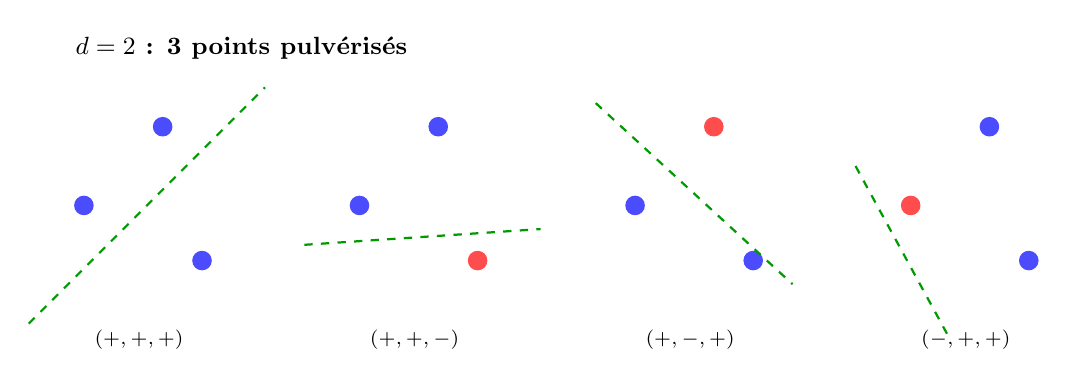
\begin{tikzpicture}[
  point/.style={circle, fill, inner sep=2pt},
  pospt/.style={circle, fill=blue!70, inner sep=2.5pt},
  negpt/.style={circle, fill=red!70, inner sep=2.5pt},
  lbl/.style={font=\scriptsize}
]
  % --- 3 points en R^2 : shattering ---
  \node[font=\small\bfseries] at (2.5, 3.5) {$d = 2$~: 3 points pulv\'eris\'es};

  % Dichotomie 1 : +++
  \begin{scope}[shift={(0,0)}]
    \node[pospt] (a1) at (0.5, 1.5) {};
    \node[pospt] (b1) at (1.5, 2.5) {};
    \node[pospt] (c1) at (2.0, 0.8) {};
    \draw[thick, green!60!black, dashed] (-0.2, 0) -- (2.8, 3.0);
    \node[lbl] at (1.2, -0.2) {$(+,+,+)$};
  \end{scope}

  % Dichotomie 2 : ++-
  \begin{scope}[shift={(3.5,0)}]
    \node[pospt] (a2) at (0.5, 1.5) {};
    \node[pospt] (b2) at (1.5, 2.5) {};
    \node[negpt] (c2) at (2.0, 0.8) {};
    \draw[thick, green!60!black, dashed] (-0.2, 1.0) -- (2.8, 1.2);
    \node[lbl] at (1.2, -0.2) {$(+,+,-)$};
  \end{scope}

  % Dichotomie 3 : +-+
  \begin{scope}[shift={(7,0)}]
    \node[pospt] (a3) at (0.5, 1.5) {};
    \node[negpt] (b3) at (1.5, 2.5) {};
    \node[pospt] (c3) at (2.0, 0.8) {};
    \draw[thick, green!60!black, dashed] (0, 2.8) -- (2.5, 0.5);
    \node[lbl] at (1.2, -0.2) {$(+,-,+)$};
  \end{scope}

  % Dichotomie 4 : -++
  \begin{scope}[shift={(10.5,0)}]
    \node[negpt] (a4) at (0.5, 1.5) {};
    \node[pospt] (b4) at (1.5, 2.5) {};
    \node[pospt] (c4) at (2.0, 0.8) {};
    \draw[thick, green!60!black, dashed] (-0.2, 2.0) -- (1.0, -0.2);
    \node[lbl] at (1.2, -0.2) {$(-,+,+)$};
  \end{scope}
\end{tikzpicture}
\end{center}

% ============================================================
\section{Bornes de g\'en\'eralisation}
\label{sec:generalization-bounds}
\index{bornes de g\'en\'eralisation}

\begin{theoreme}[Borne VC --- Vapnik \& Chervonenkis]
\label{thm:vc-bound}
Soit $\mathcal{H}$ une classe de dimension VC finie $d_{\text{VC}}$.
Pour tout $\delta > 0$, avec probabilit\'e $\geq 1 - \delta$ sur un
\'echantillon i.i.d.\ de taille $m$~:
\begin{equation}
  R(h_S) \leq \hat{R}_S(h_S) +
  \sqrt{\frac{d_{\text{VC}}\left(\ln\frac{2m}{d_{\text{VC}}} + 1\right)
  + \ln\frac{4}{\delta}}{m}}
  \label{eq:vc-bound}
\end{equation}
pour tout $h_S \in \mathcal{H}$.
\end{theoreme}

\begin{proof}[Esquisse de preuve]
La preuve repose sur trois ingr\'edients~:
\begin{enumerate}
  \item \textbf{Sym\'etrisation~:} on remplace la d\'eviation
    $|R(h) - \hat{R}_S(h)|$ par la d\'eviation entre deux \'echantillons
    fantômes (\emph{ghost sample}).
  \item \textbf{Lemme de Sauer-Shelah~:} le nombre de dichotomies
    r\'ealisables par $\mathcal{H}$ sur $m$ points est born\'e par~:
    \begin{equation}
      \Pi_{\mathcal{H}}(m) \leq \sum_{i=0}^{d_{\text{VC}}} \binom{m}{i}
      \leq \left(\frac{em}{d_{\text{VC}}}\right)^{d_{\text{VC}}}
    \end{equation}
  \item \textbf{In\'egalit\'e de concentration~:} on applique Hoeffding sur
    les variables de Rademacher, puis on contr\^ole l'union sur les
    dichotomies effectives.
\end{enumerate}
\end{proof}

\begin{lemme}[Sauer-Shelah]
\label{lem:sauer}
Si $\text{VCdim}(\mathcal{H}) = d$, alors la \textbf{fonction de croissance}
$\Pi_{\mathcal{H}}(m) = \max_{S \subset \mathcal{X}, |S|=m}
|\{(h(x_1), \ldots, h(x_m)) : h \in \mathcal{H}\}|$ satisfait~:
\begin{equation}
  \Pi_{\mathcal{H}}(m) \leq \sum_{i=0}^{d} \binom{m}{i}
\end{equation}
\end{lemme}

\begin{intuition}[title=\textbf{Interpr\'etation de la borne VC}]
La borne VC dit que l'\'ecart de g\'en\'eralisation d\'ecro\^it en
$O\!\left(\sqrt{d_{\text{VC}} / m}\right)$. Pour garantir une erreur
de g\'en\'eralisation $\leq \varepsilon$, il faut un nombre d'exemples
$m = O(d_{\text{VC}} / \varepsilon^2)$, proportionnel \`a la complexit\'e
de la classe d'hypoth\`eses.
\end{intuition}

% ============================================================
\section{Th\'eor\`eme <<~No Free Lunch~>>}
\label{sec:nfl}
\index{no free lunch}

\begin{theoreme}[No Free Lunch --- Wolpert, 1996]
\label{thm:nfl}
Soit $\mathcal{A}$ un algorithme d'apprentissage quelconque et
$\mathcal{F}$ l'ensemble de toutes les fonctions $\{0,1\}^d \to \{0,1\}$.
Pour tout algorithme $\mathcal{A}$, il existe une distribution
$\mathcal{D}$ telle que~:
\begin{enumerate}
  \item Il existe une fonction $f \in \mathcal{F}$ avec $R_{\mathcal{D}}(f) = 0$.
  \item Avec probabilit\'e $\geq 1/7$ sur le tirage de $S$ de taille $m \leq |\mathcal{X}|/2$~:
    \begin{equation}
      R_{\mathcal{D}}(\mathcal{A}(S)) \geq \frac{1}{8}
    \end{equation}
\end{enumerate}
\end{theoreme}

\begin{attention}[title=\textbf{Cons\'equences du No Free Lunch}]
\begin{itemize}
  \item Aucun algorithme n'est universellement meilleur que les autres
    \emph{sur toutes les distributions}.
  \item Les bonnes performances d'un algorithme reposent sur des
    \textbf{hypoth\`eses implicites} sur la distribution des donn\'ees
    (r\'egularit\'e, parcimonie, etc.).
  \item La s\'election de mod\`eles est donc \emph{fondamentale}~: il faut
    choisir la classe $\mathcal{H}$ adapt\'ee au probl\`eme.
\end{itemize}
\end{attention}

% ============================================================
\section{Courbes d'apprentissage}
\label{sec:learning-curves}
\index{courbes d'apprentissage}

\begin{definition}[Courbes d'apprentissage]
Les \textbf{courbes d'apprentissage} repr\'esentent l'erreur
d'entra\^inement et l'erreur de validation en fonction de la taille $m$
de l'\'echantillon d'entra\^inement.
\end{definition}

\begin{center}
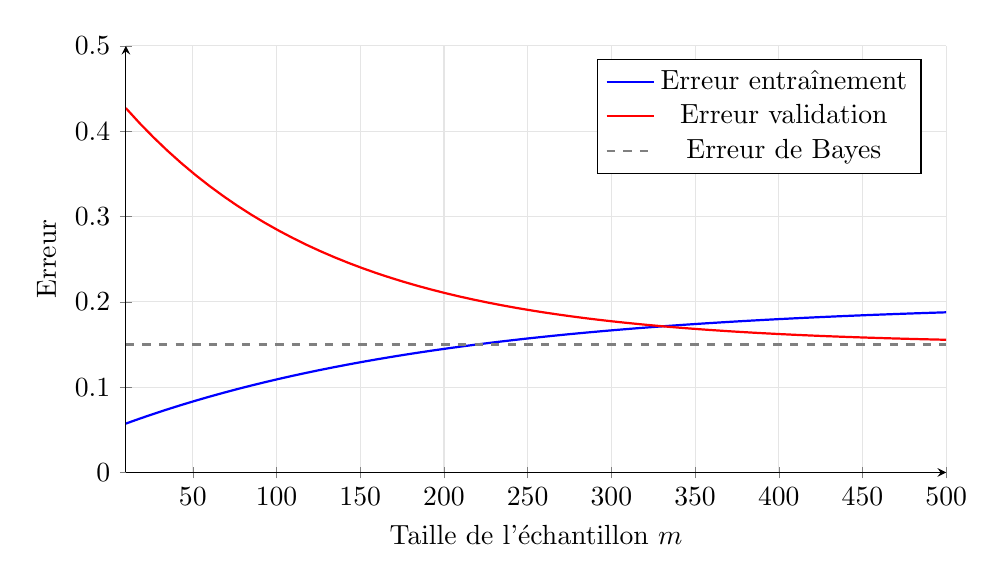
\begin{tikzpicture}
  \begin{axis}[
    width=12cm, height=7cm,
    xlabel={Taille de l'\'echantillon $m$},
    ylabel={Erreur},
    xmin=10, xmax=500, ymin=0, ymax=0.5,
    legend pos=north east,
    axis lines=left,
    grid=major, grid style={gray!20}
  ]
    % Erreur d'entrainement (croit avec m pour modele haute capacite)
    \addplot[thick, blue, domain=10:500, samples=60]
      {0.05 + 0.15*(1 - exp(-0.005*x))};
    \addlegendentry{Erreur entra\^inement}
    % Erreur de validation (decroit avec m)
    \addplot[thick, red, domain=10:500, samples=60]
      {0.15 + 0.3*exp(-0.008*x)};
    \addlegendentry{Erreur validation}
    % Erreur optimale
    \addplot[thick, gray, dashed, domain=10:500] {0.15};
    \addlegendentry{Erreur de Bayes}
  \end{axis}
\end{tikzpicture}
\end{center}

\begin{bonnepratique}[title=\textbf{Diagnostic par les courbes d'apprentissage}]
\begin{itemize}
  \item \textbf{Biais \'elev\'e (underfitting)}~: les deux courbes convergent
    vers une erreur \'elev\'ee. Ajouter des donn\'ees ne servira pas~;
    il faut augmenter la complexit\'e du mod\`ele.
  \item \textbf{Variance \'elev\'ee (overfitting)}~: grand \'ecart entre les
    courbes. Ajouter des donn\'ees ou r\'egulariser peut aider.
  \item \textbf{Bon compromis}~: les courbes convergent vers une erreur
    proche de l'erreur de Bayes.
\end{itemize}
\end{bonnepratique}

% ============================================================
\section{Impl\'ementation~: pipeline de s\'election de mod\`eles}
\label{sec:implementation-selection}

\begin{codeblock}[title=\textbf{Comparaison Grid Search, Random Search et courbes d'apprentissage}]
\begin{minted}{python}
import numpy as np
import matplotlib.pyplot as plt
from sklearn.datasets import load_breast_cancer
from sklearn.model_selection import (
    train_test_split, GridSearchCV, RandomizedSearchCV,
    learning_curve
)
from sklearn.svm import SVC
from sklearn.ensemble import RandomForestClassifier
from sklearn.preprocessing import StandardScaler
from sklearn.pipeline import Pipeline
from scipy.stats import uniform, randint

# Charger les donnees
X, y = load_breast_cancer(return_X_y=True)
X_train, X_test, y_train, y_test = train_test_split(
    X, y, test_size=0.2, random_state=42, stratify=y
)

# --- Grid Search sur SVM ---
pipe_svm = Pipeline([
    ('scaler', StandardScaler()),
    ('svm', SVC())
])
param_grid = {
    'svm__C': [0.1, 1, 10, 100],
    'svm__gamma': ['scale', 0.01, 0.001],
    'svm__kernel': ['rbf', 'poly']
}
grid = GridSearchCV(pipe_svm, param_grid, cv=5,
                    scoring='accuracy', n_jobs=-1)
grid.fit(X_train, y_train)
print(f"Grid Search - Meilleurs params: {grid.best_params_}")
print(f"Grid Search - Accuracy CV: {grid.best_score_:.4f}")
print(f"Grid Search - Accuracy test: "
      f"{grid.score(X_test, y_test):.4f}")
\end{minted}
\end{codeblock}

\begin{codeoutput}
\begin{verbatim}
Grid Search - Meilleurs params: {'svm__C': 10,
    'svm__gamma': 'scale', 'svm__kernel': 'rbf'}
Grid Search - Accuracy CV: 0.9780
Grid Search - Accuracy test: 0.9825
\end{verbatim}
\end{codeoutput}

\begin{codeblock}[title=\textbf{Random Search et courbes d'apprentissage}]
\begin{minted}{python}
# --- Random Search sur Random Forest ---
pipe_rf = Pipeline([
    ('scaler', StandardScaler()),
    ('rf', RandomForestClassifier(random_state=42))
])
param_dist = {
    'rf__n_estimators': randint(50, 300),
    'rf__max_depth': [None, 5, 10, 20, 30],
    'rf__min_samples_split': randint(2, 20),
    'rf__max_features': ['sqrt', 'log2']
}
random_search = RandomizedSearchCV(
    pipe_rf, param_dist, n_iter=50, cv=5,
    scoring='accuracy', random_state=42, n_jobs=-1
)
random_search.fit(X_train, y_train)
print(f"Random Search - Accuracy CV: "
      f"{random_search.best_score_:.4f}")
print(f"Random Search - Accuracy test: "
      f"{random_search.score(X_test, y_test):.4f}")

# --- Courbes d'apprentissage ---
train_sizes, train_scores, val_scores = learning_curve(
    grid.best_estimator_, X_train, y_train,
    train_sizes=np.linspace(0.1, 1.0, 10),
    cv=5, scoring='accuracy', n_jobs=-1
)
plt.figure(figsize=(8, 5))
plt.plot(train_sizes, train_scores.mean(axis=1),
         'o-', label="Entrainement")
plt.plot(train_sizes, val_scores.mean(axis=1),
         's-', label="Validation")
plt.xlabel("Taille d'entrainement")
plt.ylabel("Accuracy")
plt.title("Courbes d'apprentissage (SVM)")
plt.legend()
plt.grid(True, alpha=0.3)
plt.tight_layout()
plt.savefig("learning_curves.pdf")
plt.show()
\end{minted}
\end{codeblock}

\begin{codeoutput}
\begin{verbatim}
Random Search - Accuracy CV: 0.9648
Random Search - Accuracy test: 0.9649
\end{verbatim}
\end{codeoutput}

% ============================================================
\section{Exercices}
\label{sec:exercises-ch11}

\begin{exercice}[Crit\`eres d'information --- niveau 1]
On compare trois mod\`eles de r\'egression lin\'eaire sur $n = 100$
observations~:
\begin{center}
\begin{tabular}{ccc}
\toprule
Mod\`ele & $k$ (param\`etres) & $\hat{\ell}$ (log-vraisemblance) \\
\midrule
$\mathcal{M}_1$ & 3 & $-120$ \\
$\mathcal{M}_2$ & 5 & $-115$ \\
$\mathcal{M}_3$ & 10 & $-110$ \\
\bottomrule
\end{tabular}
\end{center}
\begin{enumerate}
  \item Calculer l'AIC et le BIC pour chaque mod\`ele.
  \item Quel mod\`ele est s\'electionn\'e par chaque crit\`ere~?
  \item Commenter les diff\'erences.
\end{enumerate}
\end{exercice}

\begin{exercice}[Dimension VC --- niveau 2]
\begin{enumerate}
  \item Montrer que $\text{VCdim}(\mathcal{H}) = 2$ pour la classe des
    classifieurs par intervalle $\mathcal{H} = \{\ind[a \leq x \leq b] :
    a, b \in \R\}$.
  \item Soit $\mathcal{H}_r = \{h_{a,r} : \bm{x} \mapsto
    \ind[\norm{\bm{x} - \bm{a}} \leq r]\}$ la classe des boules dans
    $\R^d$. Montrer que $\text{VCdim}(\mathcal{H}_r) = d + 1$.
  \item D\'eterminer la dimension VC de la classe des rectangles align\'es
    sur les axes dans $\R^2$.
\end{enumerate}
\end{exercice}

\begin{exercice}[Pipeline complet de s\'election --- niveau 3]
\begin{enumerate}
  \item Charger le jeu de donn\'ees \texttt{digits} de scikit-learn.
  \item Comparer au moins 4 classifieurs (k-NN, SVM, Random Forest,
    r\'egression logistique) en utilisant \texttt{GridSearchCV} ou
    \texttt{RandomizedSearchCV} pour chacun.
  \item Pour le meilleur mod\`ele, tracer les courbes d'apprentissage
    et diagnostiquer biais/variance.
  \item Impl\'ementer une optimisation bay\'esienne simple avec
    \texttt{scikit-optimize} (\texttt{BayesSearchCV}) et comparer
    le nombre d'\'evaluations n\'ecessaires.
  \item Calculer la borne de g\'en\'eralisation VC pour un classifieur
    lin\'eaire sur ce probl\`eme ($d = 64$ features). La borne est-elle
    informative avec $n = 1797$ exemples~? Discuter.
\end{enumerate}
\end{exercice}
